\chapter{Introduction}

A real world application of continuum mechanics is the study of how different elastic waves propagate in the Earth's crust. This field, called Seismology, commonly thought of as a very much applied science, stands on a large theoretical base. With applications ranging from detection of ground composition and structure\cite{https://doi.org/10.1029/95JB00259} to providing Earthquake early warnings\cite{government_of_canada_2019}, our group found interest in delving deeper into this theoretical base.

As part of venturing into this field, we identified a problem that seemed solvable and attainable within the scope of this project. The first step when taking a set of equations and making a physical model out of it is to evaluate the different effects caused by the real world onto our equations. In our case, we put the focus on what the waves propagate in during seismic events: the soil. Typically, due to the large scale of seismic events, surface elastic waves will encounter different types of soils and these soils will have considerable effects on the propagation and amplitude of waves.

Earthquakes are composed of two different types of waves: $p$-waves (compressional) and $s$-waves (shear). These two form the complex phenomenon that are seismic waves and although quite interesting, the whole of this phenomenon is larger than the scope of this project. For this reason, we have decided to focus on the compressional part of the waves created by earthquakes: the $p$-waves.

$P$-waves are named as such from the fact they are the \textit{primary} waves that are detected, due to their faster propagation than $s$-waves. In addition to being faster than $s$-waves, $p$-waves are far less destructive than $s$-waves, if destructive at all. These two properties of $p$-waves make them a natural warning for upcoming earthquakes.

The ability to accurately and automatically detect $p$-waves, as well as localizing their origin offers the chance to prevent civilian casualties by alerting nearby people at risk before the arrival of $s$-waves. With modelling of $p$-wave propagation in soil being an integral part of localizing their origin, we found the study of how these waves interface between several mediums to be relevent and of real-world use.

Specifically, the goal of this project is to model $p$-wave propagation between 2 physical media as a naive first step to a full model of $p$-wave propagation.

\begin{center}
    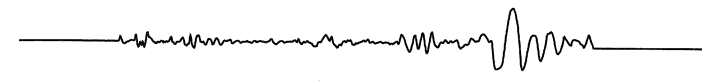
\includegraphics[width=\linewidth]{assets/trace.png}
\end{center}